% To je predloga za poročila o domačih nalogah pri predmetih, katerih
% nosilec je Blaž Zupan. Seveda lahko tudi dodaš kakšen nov, zanimiv
% in uporaben element, ki ga v tej predlogi (še) ni. Več o LaTeX-u izveš na
% spletu, na primer na http://tobi.oetiker.ch/lshort/lshort.pdf.
%
% To predlogo lahko spremeniš v PDF dokument s pomočjo programa
% pdflatex, ki je del standardne instalacije LaTeX programov.

\documentclass[a4paper,11pt]{article}
\usepackage{a4wide}
\usepackage{fullpage}
\usepackage[utf8x]{inputenc}
\usepackage[slovene]{babel}
\selectlanguage{slovene}
\usepackage[toc,page]{appendix}
\usepackage[pdftex]{graphicx} % za slike
\usepackage{setspace}
\usepackage{color}
\definecolor{light-gray}{gray}{0.95}
\usepackage{listings} % za vključevanje kode
\usepackage{hyperref}
\renewcommand{\baselinestretch}{1.2} % za boljšo berljivost večji razmak
\renewcommand{\appendixpagename}{Priloge}

\lstset{ % nastavitve za izpis kode, sem lahko tudi kaj dodaš/spremeniš
language=Python,
basicstyle=\footnotesize,
basicstyle=\ttfamily\footnotesize\setstretch{1},
backgroundcolor=\color{light-gray},
}

\title{Seštevanje sinusoid}
\author{David Rubin (david.rubin@student.um.si)}
\date{\today}

\begin{document}

\maketitle

\section{Uvod}

V programskem orodju Octave ali Python izdelajte program, ki grafično prikaže vsoto poljubnih štirih sinusoid s1, s2, s3 in s4, skupaj z izbranimi sinusoidami. Sinusoide s1, s2, s3 in s4  naj imajo interaktivno (v realnem času) nastavljivo amplitudo A, frekvenco Fr in fazo Fa. Dolžina opazovanega časovnega intervala sinusoid je lahko konstantna (npr. 1 sekunda), frekvenca vzorčenja sinusoid pa naj bo prav tako interaktivno nastavljiva.

Odgovorite na naslednja vprašanja:

\begin{enumerate}
	\item Kaj dobimo, če seštejemo sinusoidi z enako frekvenco, enako amplitudo in različno fazo?
	\item Ali lahko s seštevanjem sinusoid s1, s2, s3 in s4 dobimo neperiodičen signal?
	\item Ali lahko s seštevanjem sinusoid s1, s2,  s3 in s4 dobimo nestacionaren signal?
	\item Ali lahko s seštevanjem sinusoid s1, s2, s3 in s4 dobimo pravokotni signal?
	\item Katere vse signale, ki so našteti zgoraj ne moremo dobiti s seštevanjem sinusoid, četudi je le teh poljubno mnogo?
	\item Kakšen pa je odgovor na vprašanje 4, če so sinusoide analitične?


\end{enumerate}

\section{Poročilo}

Rešitev sem implementiral kot Python program (za delovanje potrebuje PyQt5, matplotlib in numpy), ki je priložen poročilu (\textit{main.py}).

\begin{enumerate}
	\item\textbf{Kaj dobimo, če seštejemo sinusoidi z enako frekveco, enako amplitudo in različno fazo?}

		V kolikor smo sešteli dve sinusoidi z enako frekvenco in amplitudo ter različno fazo dobimo signal, čigar faza je enaka $\varphi_1 + \varphi_2$.
	%\begin{figure}[htbp]
	%\begin{center}
	%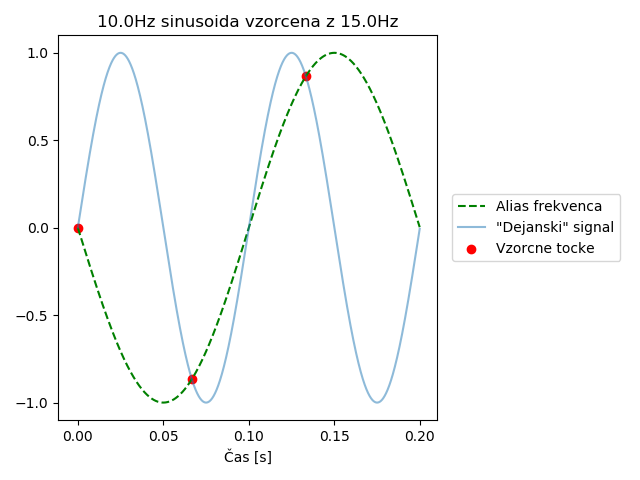
\includegraphics[scale=0.6]{alias.png}
	%\caption{Pojavitev nižje frekvence pri nezadostno visoki frekvenci vzorčenja.}
	%\label{slika1}
	%\end{center}
	%\end{figure}


 	\item \textbf{Ali lahko s seštevanjem sinusoid s1, s2, s3 in s4 dobimo neperiodičen signal?}

V kolikor seštevamo periodične signale, bo rezultat tudi periodičen signal.

 	
	\item \textbf{Ali lahko s seštevanjem sinusoid s1, s2,  s3 in s4 dobimo nestacionaren signal?}
	
Signal, ki je skupek 4 sinusoid, bo v katerem koli danem trenutku imel prisotne vse 4 frekvence posameznih sinusoid, torej ostane stacionaren in ne moremo dobiti nestacionarnega signala.	
	
	\item \textbf{Ali lahko s seštevanjem sinusoid s1, s2, s3 in s4 dobimo pravokotni signal?}

Ne, saj bi za takšen signal potrebovali neskončno mnogo sinusoid. Idealen pravokotni signal dobimo s seštevanjem lihih komponent harmonične vrste signalov (imajo obliko $2\pi (2k − 1)f$)
	
	
	\item \textbf{Katere vse signale, ki so našteti zgoraj ne moremo dobiti s seštevanjem sinusoid, četudi je le teh poljubno mnogo?}
	
Neperiodične in nestacionarne.

	\item \textbf{Kakšen pa je odgovor na vprašanje 4, če so sinusoide analitične?}

Odgovor na vprašanje 4 se v primeru analitičnih sinusoid ne spremeni.

\end{enumerate}

\end{document}
